\documentclass[UTF8,a4paper,10.5pt,fontset=windows]{ctexart}

\usepackage{geometry}
\usepackage{graphicx}
\usepackage{booktabs}
\usepackage{array}
\usepackage{float}
\usepackage{placeins}
\usepackage{xurl}
\usepackage{hyperref}
\usepackage{caption}
\usepackage{indentfirst}

\geometry{left=2.5cm,right=2.5cm,top=2.6cm,bottom=2.6cm}
\setlength{\parindent}{2em}
\setlength{\parskip}{0pt}
\emergencystretch=2em
\sloppy
\pagestyle{plain}
\captionsetup{font=small,labelsep=quad}

\newcommand{\YOLOBase}{\mbox{YOLO11n}}
\newcommand{\YOLOPtwo}{\mbox{YOLO11n-P2}}
\newcommand{\YOLOPtwoCA}{\mbox{YOLO11n-P2-CA}}
\newcommand{\YOLOPtwoCANine}{\mbox{YOLO11n-P2-CA-960}}
\newcommand{\YOLOPtwoCASmall}{\mbox{YOLO11n-P2-CA-SmallObjAug}}
\newcommand{\YOLOEightN}{\mbox{YOLOv8n}}
\newcommand{\YOLOElevenS}{\mbox{YOLO11s}}
\newcommand{\CoordAtt}{\mbox{CoordAttention}}

\title{\heiti 面向无人机航拍小目标检测的轻量化 YOLO11n 改进方法}
\author{}
\date{}

\begin{document}
\maketitle

\begin{abstract}
无人机航拍图像通常具有俯视视角、目标尺度小、分布密集、遮挡频繁和背景复杂等特点，对实时检测模型的小目标感知和定位能力提出了较高要求。针对 VisDrone 场景下的小目标检测问题，本文以 \YOLOBase{} 为基线，构建并评估了一种结合 P2 高分辨率检测分支、\CoordAtt{} 注意力机制和 960 输入分辨率的轻量化改进模型。该方法通过 P2 分支增强浅层高分辨率特征利用，通过 \CoordAtt{} 引入方向位置敏感信息，并通过较高输入分辨率提高小目标在输入图像和特征图中的有效像素占比。实验结果表明，在当前实验设置下，960 输入分辨率是性能增益的主要来源，P2 分支和 \CoordAtt{} 提供轻量级结构补充。最终，\YOLOPtwoCANine{} 在 VisDrone 验证集上取得最佳 mAP50 0.420 和 mAP50-95 0.252，较 \YOLOBase{} 基线分别提升 9.84 和 6.94 个百分点；单图推理测试达到 19.68 FPS，体现出一定的精度与速度折中。

\noindent\textbf{关键词：}无人机目标检测；小目标检测；\YOLOBase{}；\CoordAtt{}；VisDrone
\end{abstract}

\section{引言}

无人机平台已广泛应用于交通监控、应急巡检和低空遥感等场景。与地面视角图像相比，无人机航拍图像通常具有俯视视角、尺度变化显著、密集分布和背景复杂等特点。VisDrone2019-DET 数据集包含行人、车辆、非机动车等多类目标，目标尺度小且遮挡频繁，是无人机目标检测研究中的常用基准\cite{du2019visdrone}。在该类场景中，小目标像素占比较低，目标之间距离较近，容易增加定位、分类和召回难度。

YOLO 系列检测器具有端到端推理、速度快和部署方便等特点，适合实时检测任务。Ultralytics YOLO11 延续了 YOLO 系列的实时检测特性，并提供多种规模模型\cite{khanam2024yolov11,ultralytics_yolo11}。其中，\YOLOBase{} 参数量较小、推理速度较快，适合作为轻量化基线。然而，在 VisDrone 等小目标占比较高的数据集上，轻量模型可能受限于深层特征空间分辨率不足，导致小目标细节信息在多次下采样后被削弱。

为提升 \YOLOBase{} 在无人机小目标检测中的表现，本文从特征尺度、注意力表达和输入分辨率三个方面开展实验研究。主要工作如下：

\begin{enumerate}
  \item 构建 \YOLOPtwoCA{} 模型，在轻量化基线基础上引入 P2 高分辨率检测分支和 \CoordAtt{} 注意力模块，以增强浅层高分辨率特征和位置敏感表达。
  \item 系统比较 \YOLOBase{}、\YOLOPtwo{}、\YOLOPtwoCA{}、\YOLOPtwoCANine{} 和 \YOLOPtwoCASmall{}，所有数值均来自真实训练日志、验证结果文件或速度测试脚本。
  \item 从检测精度、消融实验、模型复杂度、推理速度、类别级结果和可视化案例等方面整理可复现实验材料，并补充 \YOLOEightN{} 与 \YOLOElevenS{} 外部参考基线，讨论不同改进项在当前实验设置下的作用边界。
\end{enumerate}

\section{相关工作}

\subsection{无人机航拍目标检测}

无人机航拍图像具有俯视视角、目标尺度小、密集分布、遮挡频繁和背景复杂等特点。与常规地面目标检测相比，航拍图像中的行人、非机动车和远距离车辆通常只占据较少像素，目标外观信息不足，检测器需要同时处理小尺度定位、密集目标分离和复杂背景抑制等问题。VisDrone 是无人机目标检测任务中常用的数据集，覆盖 pedestrian、people、car、motor 等多类航拍目标，能够较好反映城市交通和低空巡检场景中的检测难点\cite{du2019visdrone,ultralytics_visdrone}。

小目标和密集目标会同时增加定位、分类和召回难度。一方面，小目标在深层特征图上的有效响应区域有限，容易在下采样过程中丢失边缘和纹理信息；另一方面，密集目标之间的边界接近，检测框重叠程度较高，后处理过程也可能影响最终召回。因此，在无人机航拍检测中，如何增强浅层空间信息并保持较高推理效率，是轻量化模型设计的重要问题。

\subsection{YOLO 系列轻量化检测器}

YOLO 系列方法以端到端检测和较快推理速度为主要特点，适合实时检测和边缘部署任务。对于无人机场景，轻量模型能够降低计算开销和存储成本，但也更容易受到特征容量和空间分辨率限制。本文选择 \YOLOBase{} 作为基线，是因为其参数量较小、推理速度较快，便于在可接受复杂度下评估小目标增强策略。

轻量模型的主要问题在于深层特征图分辨率有限。经过多次下采样后，小目标在高层语义特征中的空间占比进一步降低，可能影响定位精度和召回率。因此，许多小目标检测改进会通过多尺度检测头、浅层特征融合或高分辨率输入来增强细粒度信息。本文的 P2 分支设计即沿着这一思路，将更高空间分辨率的浅层特征引入检测输出。

\subsection{小目标检测增强策略}

小目标检测常见增强策略包括高分辨率输入、多尺度检测头、浅层特征融合、注意力机制和数据增强等。高分辨率输入能够直接增加小目标在原图中的像素占比，通常对航拍小目标检测较为关键；多尺度检测头和浅层特征融合则试图在网络内部保留更多细粒度空间信息。

注意力机制能够通过重新分配特征响应提升网络表达能力。\CoordAtt{} 将位置信息嵌入通道注意力建模过程，在保持轻量化的同时引入方向感知和位置敏感特征表达\cite{hou2021coordinate}。对于无人机图像中的小目标、密集目标和复杂背景，该机制可能有助于增强目标区域响应。不过，注意力模块的实际收益需要结合消融结果谨慎判断。本文实验显示，\CoordAtt{} 在 P2 基础上带来的是小幅补充提升，而非主要增益来源。

数据增强也可能影响小目标检测效果，例如 mosaic 关闭时机、缩放范围、copy-paste 和 erasing 等设置均会改变训练样本分布。本文保留小目标友好增强作为训练策略消融，但当前结果显示该策略未超过 \YOLOPtwoCA{}，说明增强策略需要与数据集分布和模型结构进一步匹配。

\section{方法}

本文方法以 \YOLOBase{} 为基础，整体包含三项设计：第一，引入 P2 高分辨率检测分支，使检测输出由原始 P3/P4/P5 扩展为 P2/P3/P4/P5；第二，在特征融合分支中加入 \CoordAtt{}，以较低额外开销补充方向位置敏感建模；第三，在 \YOLOPtwoCA{} 基础上采用 960 输入分辨率进行高分辨率小目标检测实验。整体设计仍保持轻量化模型规模，具体结构差异如表 \ref{tab:structure_diff} 所示。

\begin{table}[htbp]
\centering
\caption{\YOLOBase{} 与改进模型的结构差异对比}
\label{tab:structure_diff}
\small
\begin{tabular}{p{0.18\textwidth}p{0.34\textwidth}p{0.38\textwidth}}
\toprule
模块 & 原始 \YOLOBase{} & 改进模型 \\
\midrule
检测尺度 & P3/P4/P5 & P2/P3/P4/P5 \\
小目标特征 & 主要依赖较深层特征 & 引入浅层高分辨率特征 \\
注意力模块 & 无 & 在特征融合分支后加入 \CoordAtt{} \\
输入尺寸 & 640 & 960 \\
输出目标 & 常规实时检测 & 面向无人机小目标检测的精度--速度折中 \\
\bottomrule
\end{tabular}
\end{table}

\begin{figure}[htbp]
\centering
\small
\setlength{\tabcolsep}{4pt}
\begin{tabular}{c}
\fbox{\strut 输入图像 960} \\
$\downarrow$ \\
\fbox{\strut \YOLOBase{} Backbone} \\
$\downarrow$ \\
\fbox{\strut Neck / Feature Fusion} \\
$\downarrow$ \\
\fbox{\strut P2/P3/P4/P5 四尺度特征} \\
$\downarrow$ \\
\fbox{\strut \CoordAtt{} 位置敏感增强} \\
$\downarrow$ \\
\fbox{\strut Detect Head} \\
$\downarrow$ \\
\fbox{\strut 检测结果}
\end{tabular}
\caption{\YOLOPtwoCANine{} 结构示意图}
\label{fig:method_overview}
\end{figure}

\subsection{P2 高分辨率检测分支}

原始 \YOLOBase{} 主要依赖 P3/P4/P5 检测尺度。对于 VisDrone 中大量远距离行人、车辆和非机动车目标，目标在多次下采样后容易在深层特征图中丢失细节。为缓解该问题，本文在 \YOLOBase{} 检测头中加入 P2 高分辨率检测分支，使模型能够利用更浅层、更高空间分辨率的特征进行预测。改进后模型采用 P2/P3/P4/P5 四尺度输出，从而提高小尺度目标在特征图中的可见性。具体实现配置见项目中的 \texttt{yolo11n\_p2.yaml}。

\subsection{\CoordAtt{} 注意力增强}

在 P2 模型基础上，本文进一步加入 \CoordAtt{} 模块。\CoordAtt{} 在建模通道关系的同时保留方向位置信息，有助于模型在复杂背景下补充位置敏感特征表达。对于无人机航拍图像中的小目标和密集目标，该模块可能增强目标区域与背景区域的区分能力。需要强调的是，结合后续消融结果，\CoordAtt{} 带来的收益幅度有限，主要作为 P2 结构后的轻量级补充增强模块。具体实现配置见项目中的 \texttt{yolo11n\_p2\_coordatt.yaml}。

\subsection{高分辨率输入与小目标友好增强}

由于 VisDrone 中小目标占比较高，输入分辨率会直接影响目标在图像和中间特征图中的像素占比。本文在 \YOLOPtwoCA{} 基础上测试 960 输入分辨率。当前实验结果显示，960 输入分辨率带来的提升最明显，是本文已完成实验中的主要增益来源。

此外，本文设计了小目标友好数据增强消融实验，设置包括 \texttt{close\_mosaic: 20}、\texttt{scale: 0.35}、\texttt{copy\_paste: 0.1} 和 \texttt{erasing: 0.0}。其中，较早关闭 mosaic 用于减少训练后期合成图像分布影响，较小 scale 用于降低小目标被过度缩小的风险，关闭 erasing 用于避免破坏小目标可见区域。当前结果显示该增强策略未超过 \YOLOPtwoCA{}，因此本文仅将其作为训练策略消融进行讨论。

\section{实验与分析}

\subsection{实验设置}

实验基于 Ultralytics YOLO 框架，在 VisDrone2019-DET 数据集上进行。数据配置文件为 \texttt{configs/dataset/visdrone.yaml}，训练集、验证集和 test-dev 图像均转换为 YOLO 格式组织。所有已完成主实验均训练 100 个 epoch，并使用各实验输出目录中的 \texttt{results.csv} 统计最终指标与最佳指标。当前未获得 VisDrone 官方 test-dev/test-challenge 返回结果，因此本文仅报告验证集结果。

实验环境与训练配置如表 \ref{tab:env} 所示。表中版本信息由当前本地环境命令自动检测得到；训练轮数、输入尺寸、batch size、随机种子和优化器设置来自训练配置、\texttt{args.yaml} 或训练日志。

\begin{table}[htbp]
\centering
\caption{实验环境与训练配置}
\label{tab:env}
\small
\begin{tabular}{p{0.30\textwidth}p{0.58\textwidth}}
\toprule
项目 & 设置 \\
\midrule
数据集 & VisDrone2019-DET \\
训练轮数 & 100 epochs \\
输入尺寸 & 640 / 960 \\
GPU & 本地测速环境为 NVIDIA GeForce RTX 4060 Laptop GPU, 8 GB；外部基线训练使用租用服务器 NVIDIA GeForce RTX 4090 D \\
CUDA 版本 & 12.8 \\
Python 版本 & 3.12.7 \\
PyTorch 版本 & 2.7.0+cu128 \\
Ultralytics 版本 & 8.4.51 \\
batch size & 640 输入为 8，960 输入为 4 \\
optimizer & auto；训练日志中由 Ultralytics 自动选择 \\
初始学习率 & lr0=0.01；当 optimizer=auto 时由 Ultralytics 接管 \\
% P2 系列初始化依据 runs/logs/yolo11n_p2*.log 中的 YOLO11-to-P2 remapping 记录。
预训练权重 & \YOLOBase{} 使用 \texttt{yolo11n.pt}；P2 系列基于 \texttt{yolo11n.pt} 进行可匹配层初始化，新增层随机初始化 \\
随机种子 & 42 \\
验证图像处理 & 按 Ultralytics 验证流程进行 resize/letterbox 处理 \\
NMS 设置 & 采用 Ultralytics 默认验证流程；现有日志记录 \texttt{conf=None}、\texttt{iou=0.7}、\texttt{agnostic\_nms=False} \\
速度测试 & GPU 单图 \texttt{model.predict} wall-clock 计时，10 次预热、100 张样本，并记录 Ultralytics preprocess/inference/postprocess 时间 \\
\bottomrule
\end{tabular}
\end{table}

\subsection{主实验结果}

表 \ref{tab:main_results} 给出了不同模型在 VisDrone 验证集上的检测结果。引入 P2 检测头后，最佳 mAP50 从 0.322 提升到 0.330，最佳 mAP50-95 从 0.182 提升到 0.190，说明浅层高分辨率特征对无人机小目标检测有一定帮助。加入 \CoordAtt{} 后，最佳 mAP50 和 mAP50-95 分别达到 0.331 和 0.190，较 P2 模型继续小幅提升。进一步将输入尺寸提升至 960 后，\YOLOPtwoCANine{} 取得当前已完成 \YOLOBase{} 主线实验中的最佳性能，mAP50 为 0.420，mAP50-95 为 0.252。该结果表明，在当前实验设置下，高分辨率输入是性能提升的主要来源。

\begin{table}[htbp]
\centering
\caption{不同模型在 VisDrone 验证集上的检测结果对比}
\label{tab:main_results}
\small
\resizebox{\textwidth}{!}{%
\begin{tabular}{lccccccc}
\toprule
方法 & 输入尺寸 & Params/M & GFLOPs@640 & P & R & mAP50 & mAP50-95 \\
\midrule
\YOLOBase{} & 640 & 2.592 & 6.5 & 0.454 & 0.339 & 0.322 & 0.182 \\
\YOLOPtwo{} & 640 & 2.894 & 10.7 & 0.448 & 0.355 & 0.330 & 0.190 \\
\YOLOPtwoCA{} & 640 & 2.904 & 10.7 & 0.454 & 0.350 & 0.331 & 0.190 \\
\YOLOPtwoCANine{} & 960 & 2.904 & 10.7 & 0.534 & 0.428 & 0.420 & 0.252 \\
\YOLOPtwoCASmall{} & 640 & 2.904 & 10.7 & 0.452 & 0.348 & 0.328 & 0.187 \\
\bottomrule
\end{tabular}
}
\end{table}

表中 GFLOPs@640 表示模型结构在 640 输入尺寸下的统计结果。对于 960 输入实验，实际计算量会随输入分辨率增加；由于当前已有日志仅可靠记录 640 统计值，本文不将 10.7 GFLOPs 表述为 960 输入下的实际计算量。

\subsection{外部参考基线对比}

为避免仅在 \YOLOBase{} 内部进行比较带来的局限，本文补充训练了 \YOLOEightN{} 和 \YOLOElevenS{} 两个外部参考基线，结果如表 \ref{tab:external_baseline} 所示。其中，\YOLOEightN{} 用于提供常见轻量 YOLO 模型参考，\YOLOElevenS{} 用于观察更大模型容量对 VisDrone 验证集结果的影响。需要说明的是，表 \ref{tab:external_baseline} 并不作为 P2 分支、\CoordAtt{} 或 960 输入分辨率的单因素消融依据，因为这些模型在基础架构、参数量和输入设置上并不完全一致。

从结果看，\YOLOEightN{} 与 \YOLOBase{} 的性能接近，其最佳 mAP50 和 mAP50-95 分别为 0.325 和 0.184，略高于 \YOLOBase{} 的 0.322 和 0.182。\YOLOElevenS{} 的最佳 mAP50 和 mAP50-95 分别达到 0.389 和 0.227，明显高于 nano 级基线，说明增加模型容量能够提升 VisDrone 检测精度。但 \YOLOElevenS{} 的参数量约为 9.432M，高于 \YOLOPtwoCANine{} 的 2.904M；而 \YOLOPtwoCANine{} 在更高输入分辨率下取得 0.420 mAP50 和 0.252 mAP50-95。该结果说明本文最终模型体现的是结构增强与高分辨率输入共同作用下的整体效果，而不能简单解释为单个模块相对外部基线的绝对优势。

\begin{table}[htbp]
\centering
\caption{外部参考基线在 VisDrone 验证集上的结果}
\label{tab:external_baseline}
\small
\resizebox{\textwidth}{!}{%
\begin{tabular}{lcccccc}
\toprule
方法 & 输入尺寸 & Params/M & GFLOPs@640 & P & R & mAP50 / mAP50-95 \\
\midrule
\YOLOEightN{} baseline & 640 & 3.013 & 8.2 & 0.448 & 0.346 & 0.325 / 0.184 \\
\YOLOElevenS{} baseline & 640 & 9.432 & 21.6 & 0.524 & 0.393 & 0.389 / 0.227 \\
\YOLOBase{} baseline & 640 & 2.592 & 6.5 & 0.454 & 0.339 & 0.322 / 0.182 \\
\YOLOPtwoCANine{} & 960 & 2.904 & 10.7 & 0.534 & 0.428 & 0.420 / 0.252 \\
\bottomrule
\end{tabular}
}
\end{table}

\begin{figure}[htbp]
\centering
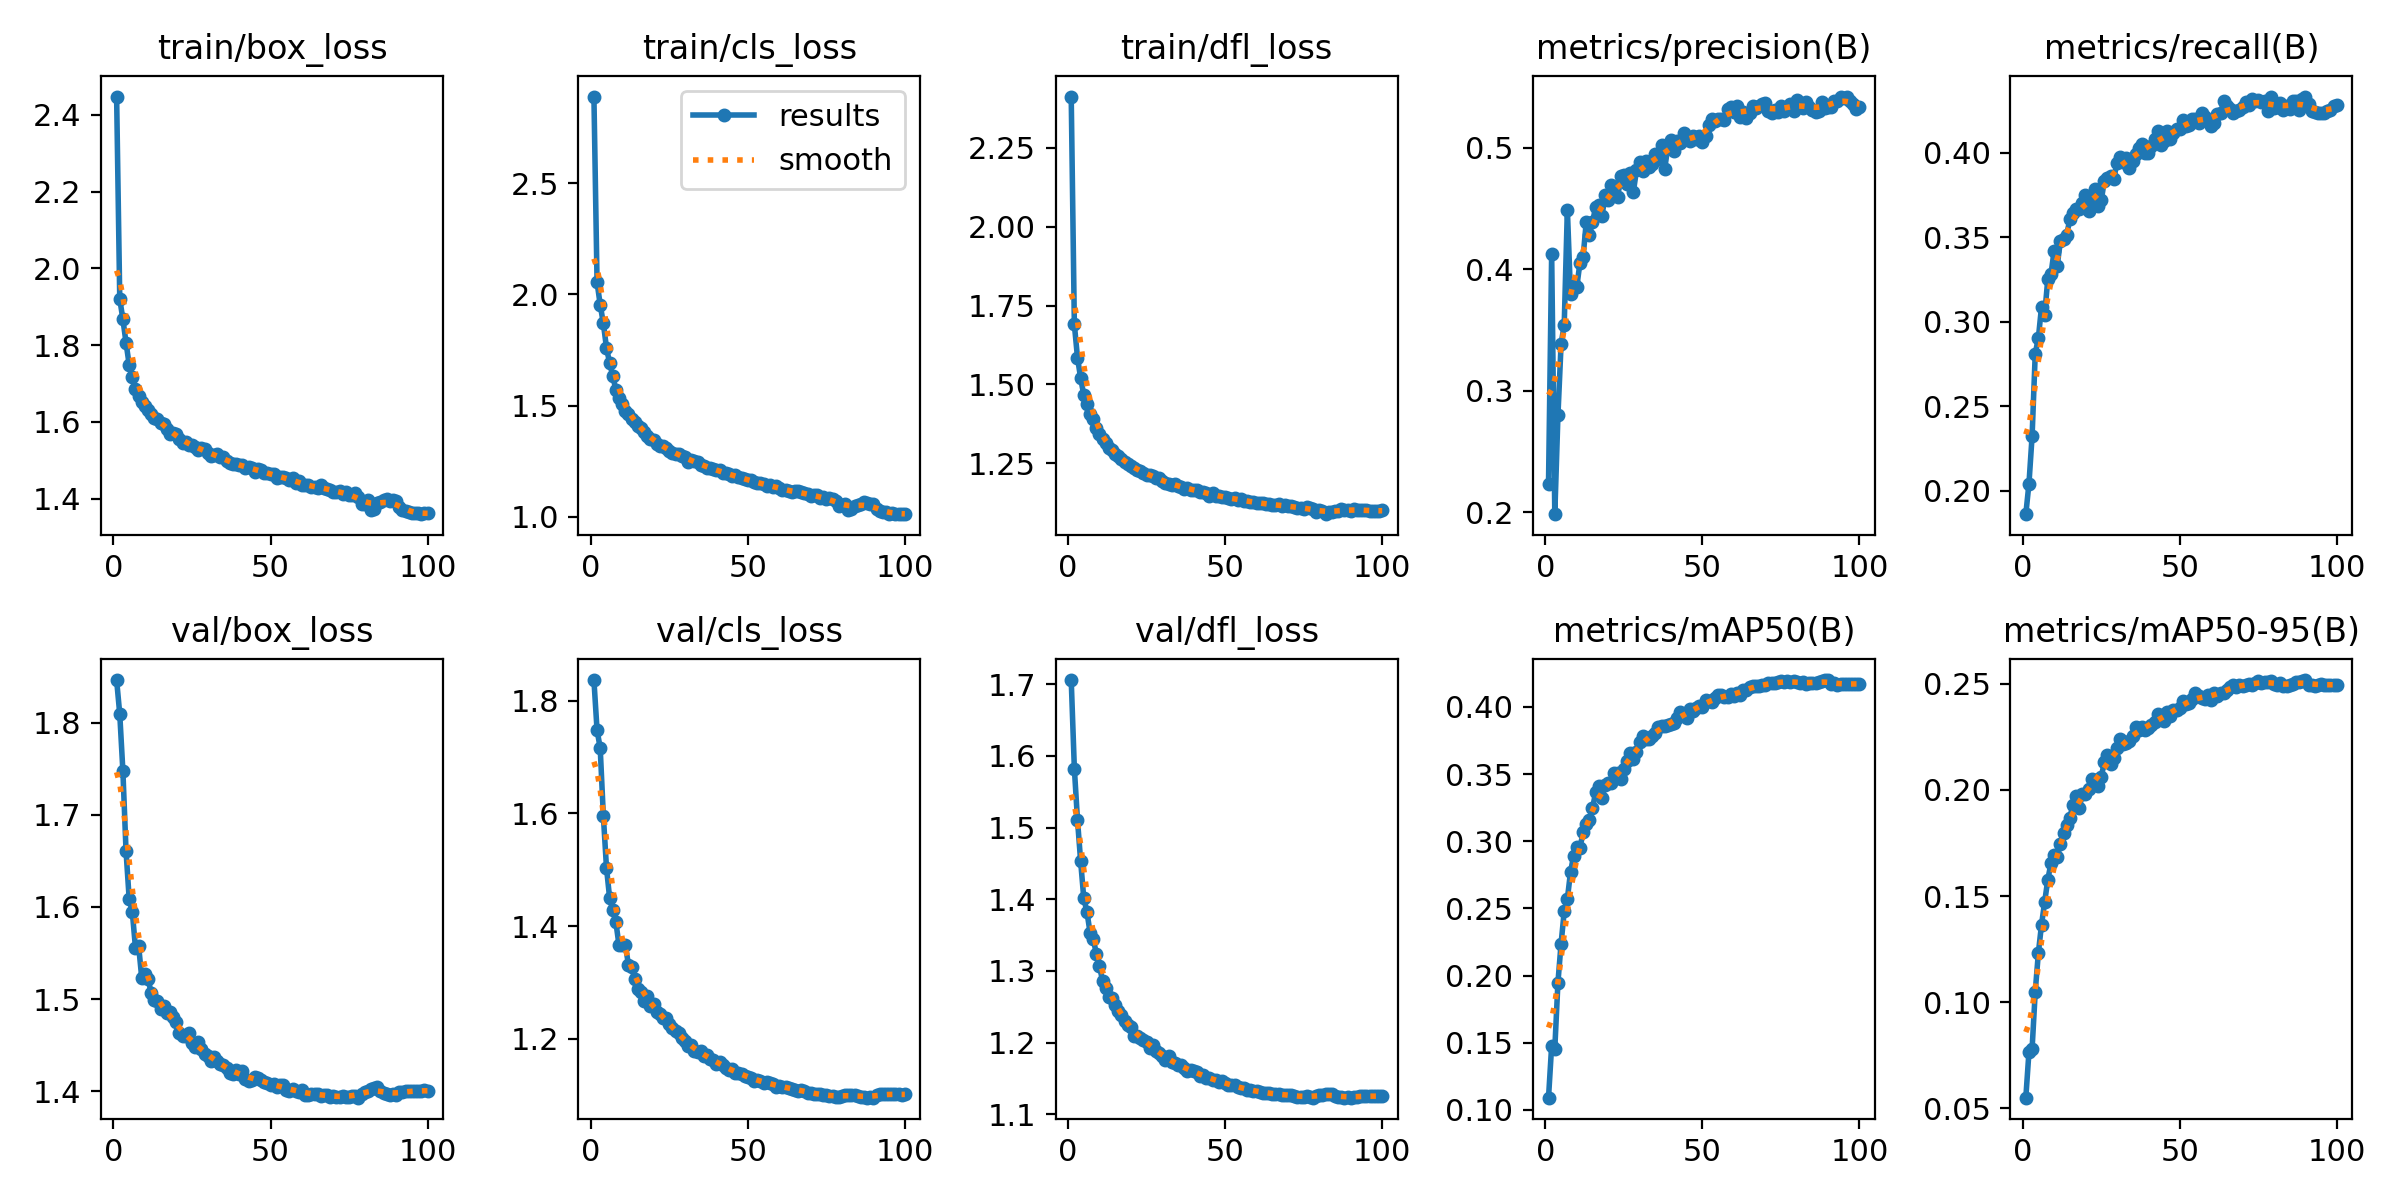
\includegraphics[width=0.95\linewidth]{figures/training_curves/p2_coordatt_960_results.png}
\caption{\YOLOPtwoCANine{} 训练与验证曲线}
\label{fig:training_curve}
\end{figure}

\subsection{消融实验}

表 \ref{tab:ablation} 展示了各改进项相对基线模型的贡献。P2 分支带来 0.009 的 mAP50 提升和 0.008 的 mAP50-95 提升，说明浅层高分辨率特征对小目标检测具有积极作用。\CoordAtt{} 在 P2 基础上继续带来小幅提升，但提升幅度有限，说明其更适合作为补充增强模块。960 输入分辨率带来的提升最明显，相对基线 mAP50 提升 9.84 个百分点，mAP50-95 提升 6.94 个百分点，进一步说明高分辨率输入是当前实验设置下性能提升的主要来源。小目标友好增强相较基线有一定提升，但未超过 P2 和 \YOLOPtwoCA{}，表明该增强策略在当前超参数下并非最优。

\begin{table}[htbp]
\centering
\caption{改进模块消融实验结果}
\label{tab:ablation}
\small
\resizebox{\textwidth}{!}{%
\begin{tabular}{llccccc}
\toprule
方法 & 改动 & 输入尺寸 & mAP50 & $\Delta$mAP50 & mAP50-95 & $\Delta$mAP50-95 \\
\midrule
\YOLOBase{} & 基线模型 & 640 & 0.322 & +0.000 & 0.182 & +0.000 \\
\YOLOPtwo{} & 增加 P2 检测头 & 640 & 0.330 & +0.009 & 0.190 & +0.008 \\
\YOLOPtwoCA{} & 增加 \CoordAtt{} & 640 & 0.331 & +0.009 & 0.190 & +0.008 \\
\YOLOPtwoCANine{} & 输入尺寸提升至 960 & 960 & 0.420 & +0.098 & 0.252 & +0.069 \\
\YOLOPtwoCASmall{} & 小目标友好增强 & 640 & 0.328 & +0.006 & 0.187 & +0.005 \\
\bottomrule
\end{tabular}
}
\end{table}

\subsection{小目标尺度分布与召回分析}

为进一步验证 VisDrone 场景中小目标占比较高这一问题设定，本文基于 YOLO 格式标注文件统计训练集和验证集目标框面积分布。尺度划分采用常见的 COCO 面积阈值：small 表示目标框面积小于 $32^2$ 像素，medium 表示面积位于 $32^2$ 至 $96^2$ 像素之间，large 表示面积不小于 $96^2$ 像素。统计结果如表 \ref{tab:scale_distribution} 和图 \ref{fig:scale_distribution} 所示。验证集中 small 目标共有 26586 个，占全部验证集标注实例的 68.59\%；训练集中 small 目标共有 207604 个，占比 60.49\%。这说明 VisDrone 验证集具有明显的小目标主导特征，也解释了高分辨率输入和 P2 高分辨率检测分支对该任务的重要性。

\begin{table}[htbp]
\centering
\caption{VisDrone YOLO 格式标注中的目标尺度分布}
\label{tab:scale_distribution}
\small
\begin{tabular}{lrrrr}
\toprule
数据划分 & small & medium & large & small 占比 \\
\midrule
train & 207604 & 116620 & 18980 & 60.49\% \\
val & 26586 & 11105 & 1068 & 68.59\% \\
\bottomrule
\end{tabular}
\end{table}

\begin{figure}[htbp]
\centering
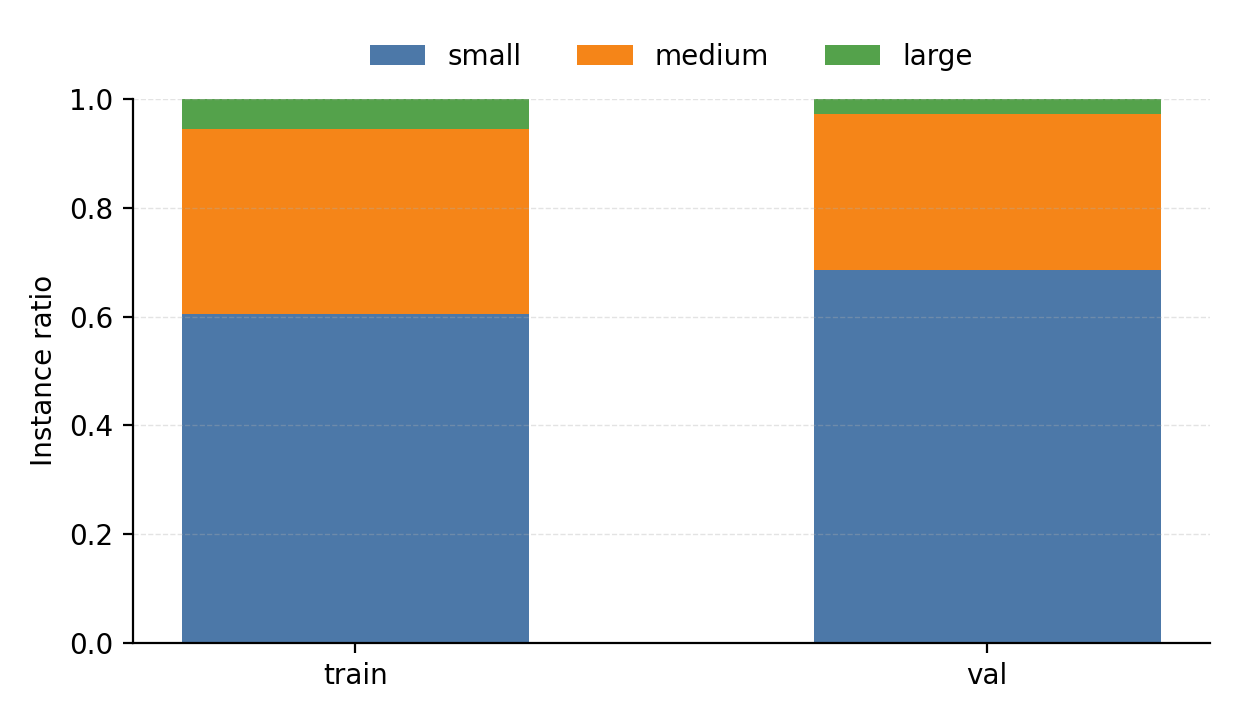
\includegraphics[width=0.78\linewidth]{figures/scale_analysis/object_scale_distribution.png}
\caption{VisDrone 训练集和验证集目标尺度分布}
\label{fig:scale_distribution}
\end{figure}

在此基础上，本文进一步使用验证集预测结果进行尺度分组匹配分析。该分析采用 \texttt{conf=0.25} 和 IoU=0.5 的阈值设置，将预测框与同类别标注框进行一对一匹配，并按标注框尺度统计召回率和预测精度。需要说明的是，该结果用于分析不同尺度目标的匹配情况，并不等同于官方 AP 指标。结果如表 \ref{tab:scale_group_results} 和图 \ref{fig:scale_group_recall} 所示。与 \YOLOBase{} 相比，\YOLOPtwoCANine{} 在 small 目标上的召回率由 0.308 提升至 0.455，提升幅度为 14.74 个百分点；medium 目标召回率由 0.712 提升至 0.781；large 目标召回率变化较小。该结果表明，最终模型的主要收益集中在 small 和 medium 目标，符合本文面向无人机航拍小目标检测的设计目标。

\begin{table}[htbp]
\centering
\caption{不同尺度目标的验证集匹配结果}
\label{tab:scale_group_results}
\small
\resizebox{\textwidth}{!}{%
\begin{tabular}{lcrrrrr}
\toprule
模型 & 尺度 & 标注实例数 & 匹配标注数 & Recall@0.5 & 预测数 & Precision@0.5 \\
\midrule
\YOLOBase{} & small & 26586 & 8180 & 0.308 & 12844 & 0.633 \\
\YOLOBase{} & medium & 11105 & 7906 & 0.712 & 10472 & 0.759 \\
\YOLOBase{} & large & 1068 & 929 & 0.870 & 1080 & 0.866 \\
\YOLOPtwoCANine{} & small & 26586 & 12099 & 0.455 & 17981 & 0.666 \\
\YOLOPtwoCANine{} & medium & 11105 & 8678 & 0.781 & 11144 & 0.789 \\
\YOLOPtwoCANine{} & large & 1068 & 942 & 0.882 & 1125 & 0.844 \\
\bottomrule
\end{tabular}
}
\end{table}

\begin{figure}[htbp]
\centering
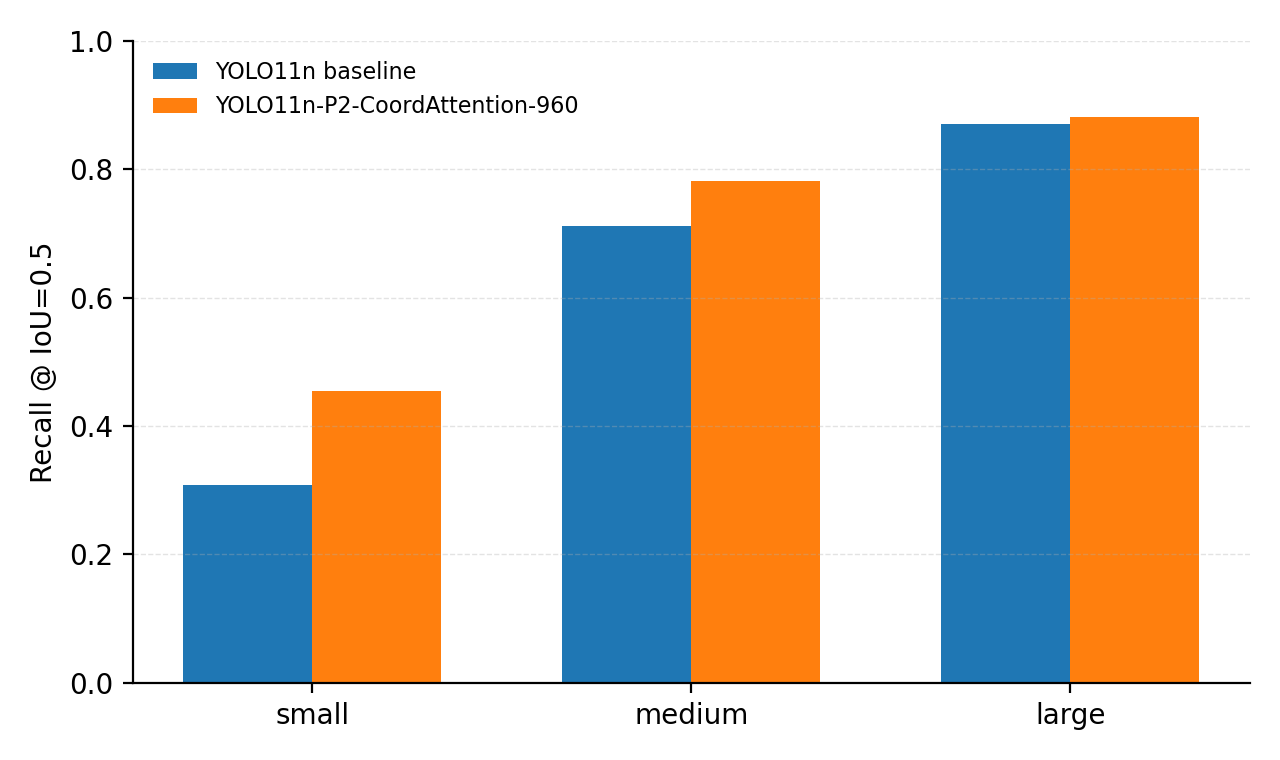
\includegraphics[width=0.78\linewidth]{figures/scale_analysis/scale_group_recall.png}
\caption{\YOLOBase{} 与 \YOLOPtwoCANine{} 在不同尺度目标上的召回率对比}
\label{fig:scale_group_recall}
\end{figure}

\subsection{类别级结果分析}

项目中已整理每类指标和验证日志，因此本文进一步给出 \YOLOPtwoCANine{} 的类别级结果，如表 \ref{tab:per_class} 所示。car、bus 和 motor 等类别的 mAP50 相对较高，说明在目标外观较稳定或实例数量较多时模型更容易学习有效特征。bicycle、tricycle 和 awning-tricycle 的 mAP50 较低，可能与非机动车在俯视视角下外观相似、实例尺度较小和遮挡较多有关。pedestrian 与 people 两类也存在一定混淆风险，这与人体目标在航拍视角下尺度小、姿态信息不足有关。

\begin{table}[htbp]
\centering
\caption{\YOLOPtwoCANine{} 在 VisDrone 验证集上的类别级结果}
\label{tab:per_class}
\small
\resizebox{\textwidth}{!}{%
\begin{tabular}{lrrrrrr}
\toprule
类别 & 图像数 & 实例数 & P & R & mAP50 & mAP50-95 \\
\midrule
pedestrian & 520 & 8844 & 0.580 & 0.501 & 0.513 & 0.243 \\
people & 482 & 5125 & 0.586 & 0.379 & 0.393 & 0.157 \\
bicycle & 364 & 1287 & 0.335 & 0.221 & 0.171 & 0.076 \\
car & 515 & 14064 & 0.736 & 0.830 & 0.837 & 0.590 \\
van & 421 & 1975 & 0.528 & 0.460 & 0.455 & 0.321 \\
truck & 266 & 750 & 0.538 & 0.395 & 0.375 & 0.249 \\
tricycle & 337 & 1045 & 0.435 & 0.317 & 0.268 & 0.155 \\
awning-tricycle & 220 & 532 & 0.300 & 0.198 & 0.133 & 0.086 \\
bus & 131 & 251 & 0.726 & 0.518 & 0.546 & 0.408 \\
motor & 485 & 4886 & 0.568 & 0.543 & 0.520 & 0.239 \\
\bottomrule
\end{tabular}
}
\end{table}

\subsection{推理速度与模型复杂度}

表 \ref{tab:speed} 给出了不同模型的复杂度和推理速度。所有速度结果均由 \texttt{tools/benchmark\_speed.py} 在同一台本地 GPU 上重新测试得到，采用单图 \texttt{model.predict} wall-clock 计时，包含预处理、推理和后处理开销。原始 \YOLOBase{} 的平均延迟为 40.09 ms，FPS 为 24.94。\YOLOPtwoCA{} 在 640 输入下平均延迟为 45.77 ms，FPS 为 21.85，说明 P2 分支和注意力模块会带来一定额外开销。\YOLOPtwoCANine{} 的平均延迟为 50.81 ms，FPS 为 19.68。虽然 960 输入降低了推理速度，但其验证集精度提升更明显，因此更适合对小目标检测精度要求较高且仍需保持一定推理效率的场景。

\begin{table}[htbp]
\centering
\caption{不同模型复杂度与推理速度对比}
\label{tab:speed}
\small
\resizebox{\textwidth}{!}{%
\begin{tabular}{lcccccc}
\toprule
方法 & 输入尺寸 & Params/M & GFLOPs@640 & 权重/MB & 平均延迟/ms & FPS \\
\midrule
\YOLOEightN{} baseline & 640 & 3.013 & 8.2 & 5.95 & 42.29 & 23.65 \\
\YOLOElevenS{} baseline & 640 & 9.432 & 21.6 & 18.28 & 38.97 & 25.66 \\
\YOLOBase{} & 640 & 2.592 & 6.5 & 5.21 & 40.09 & 24.94 \\
\YOLOPtwo{} & 640 & 2.894 & 10.7 & 5.91 & 43.64 & 22.91 \\
\YOLOPtwoCA{} & 640 & 2.904 & 10.7 & 5.94 & 45.77 & 21.85 \\
\YOLOPtwoCASmall{} & 640 & 2.904 & 10.7 & 5.94 & 49.96 & 20.02 \\
\YOLOPtwoCANine{} & 960 & 2.904 & 10.7 & 6.09 & 50.81 & 19.68 \\
\bottomrule
\end{tabular}
}
\end{table}

\subsection{可视化分析}

图 \ref{fig:qualitative} 展示了 \YOLOPtwoCANine{} 在 VisDrone 验证集上的检测示例。模型在一般密集交通场景下能够检测出多类车辆、行人和非机动车目标。图 \ref{fig:failure} 给出了复杂场景下的困难样例，可以观察到远距离极小目标、密集遮挡和类别外观相近仍可能导致漏检或误检。这些现象说明，尽管高分辨率输入和 P2 分支改善了小目标检测表现，复杂航拍场景中的极小目标召回和细粒度类别区分仍有进一步提升空间。

\begin{figure}[htbp]
\centering
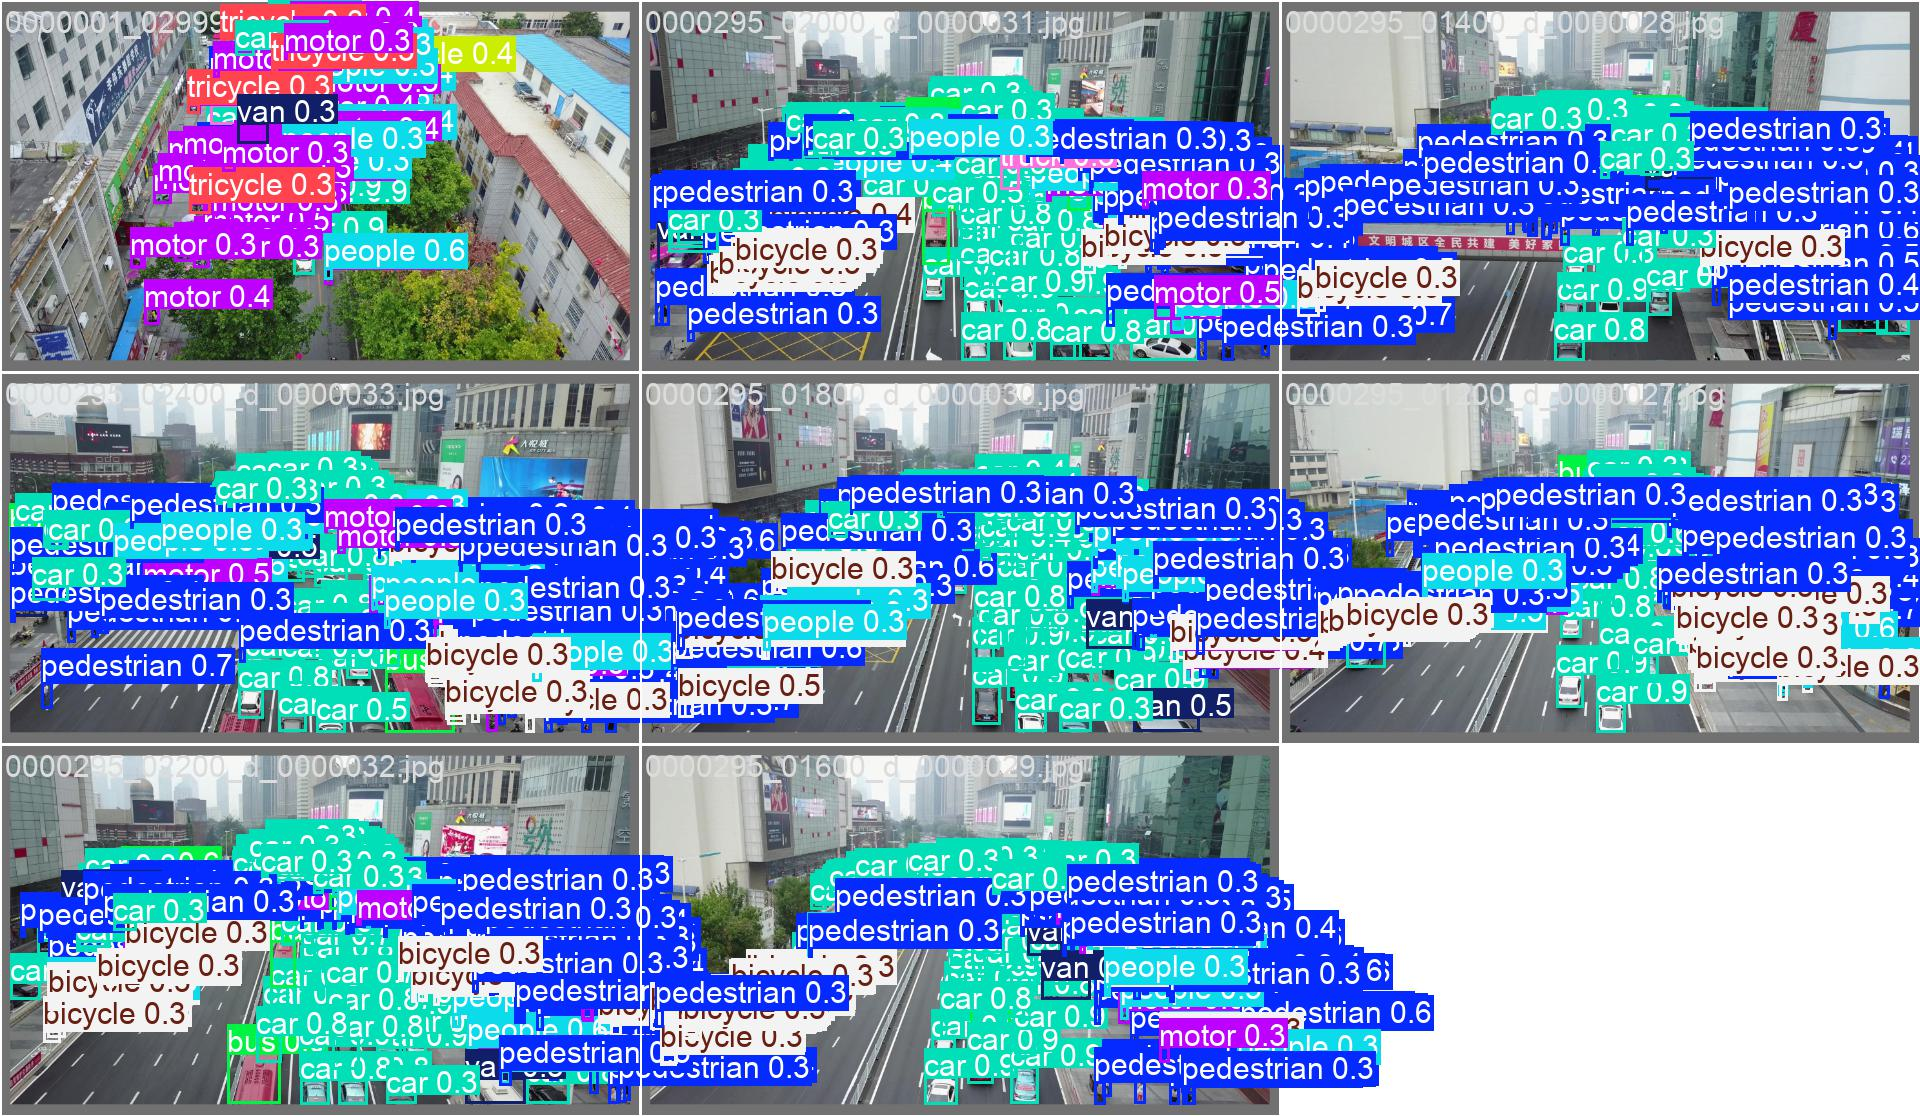
\includegraphics[width=0.82\linewidth]{figures/qualitative/p2_coordatt_960_val_batch0_pred.jpg}
\caption{VisDrone 验证集密集交通场景检测示例}
\label{fig:qualitative}
\end{figure}

\begin{figure}[htbp]
\centering
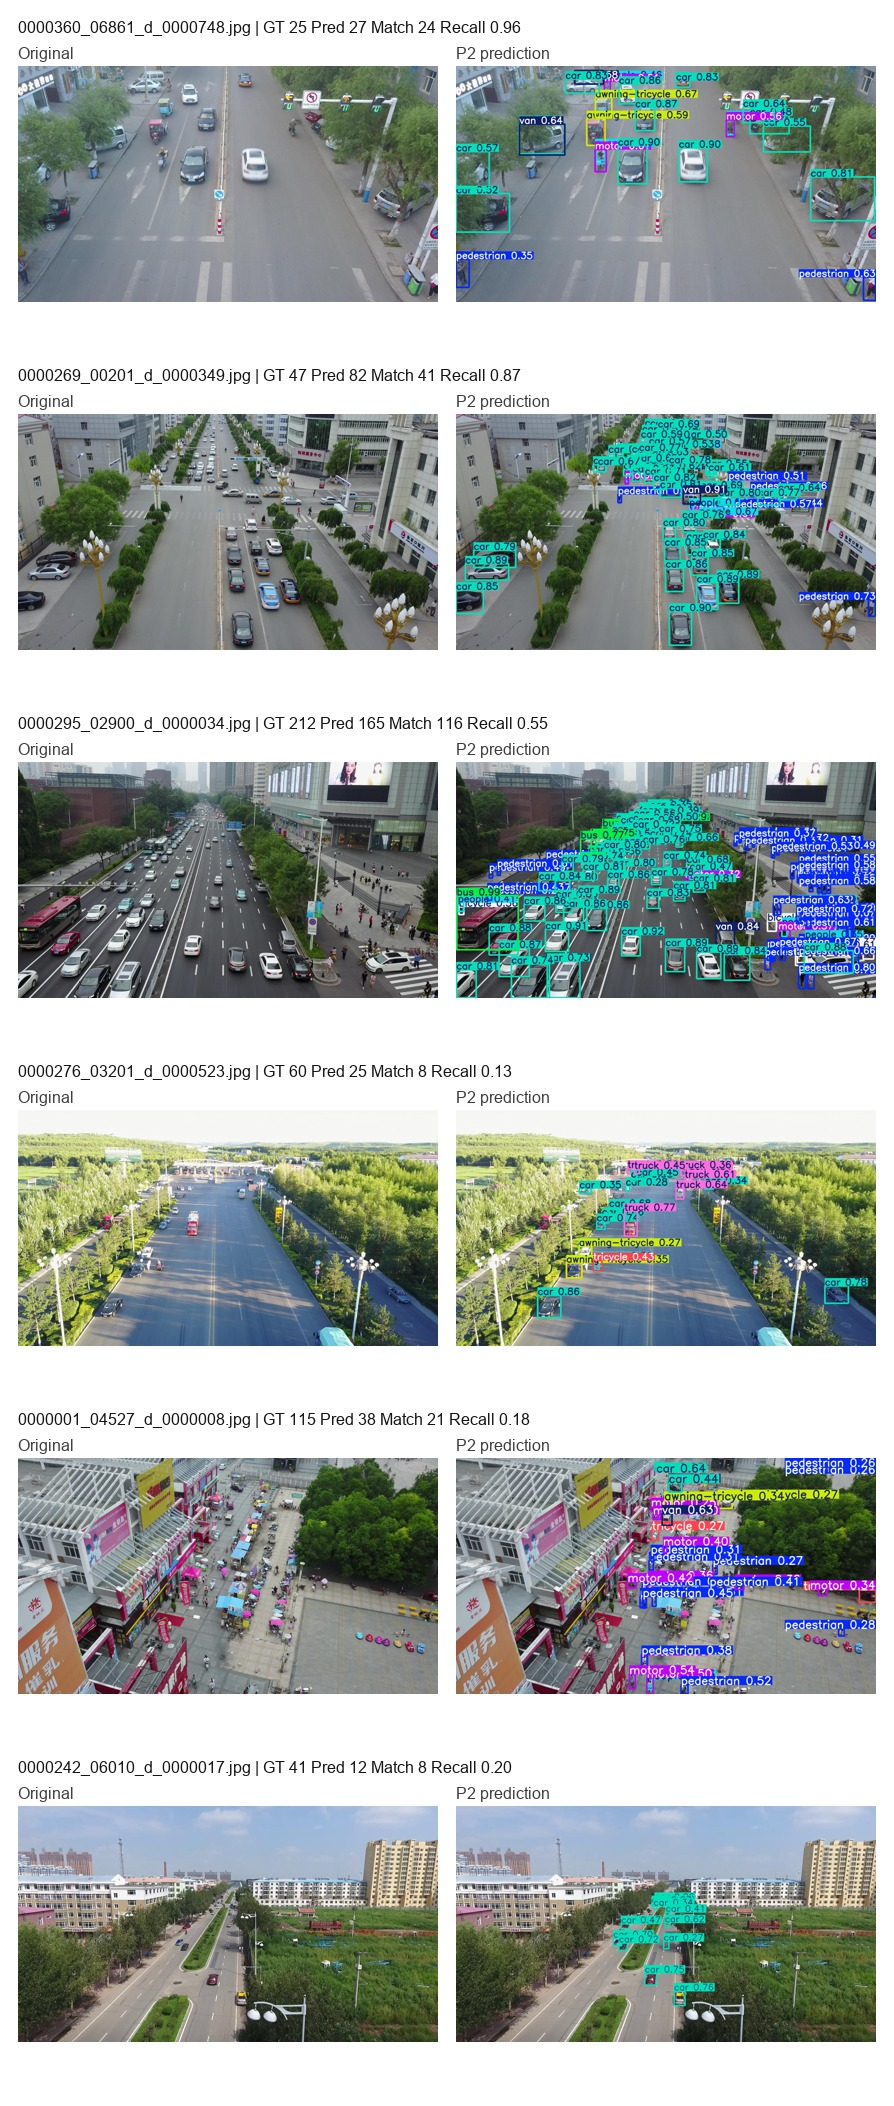
\includegraphics[height=0.65\textheight,keepaspectratio]{figures/failure_cases/p2_case_contact_sheet.jpg}
\caption{复杂场景下极小目标、密集遮挡和类别混淆示例}
\label{fig:failure}
\end{figure}

\begin{table}[htbp]
\centering
\caption{复杂场景中的典型误检与漏检原因分析}
\label{tab:failure_reason}
\small
\begin{tabular}{p{0.34\textwidth}p{0.54\textwidth}}
\toprule
失败类型 & 可能原因 \\
\midrule
远距离极小目标漏检 & 目标像素过少，纹理和边缘信息不足 \\
密集车辆遮挡 & 目标间距小，定位框重叠，NMS 后处理可能影响召回 \\
pedestrian / people 混淆 & 俯视视角下人体外观差异较小，类别边界不清晰 \\
bicycle / motor 混淆 & 非机动车在航拍视角下轮廓相似 \\
背景误检 & 道路标识、树影或车辆局部纹理可能干扰分类 \\
\bottomrule
\end{tabular}
\end{table}

\FloatBarrier

\section{讨论}

从当前已完成实验看，输入分辨率、浅层高分辨率特征和模型容量均会影响 VisDrone 航拍小目标检测效果。首先，960 输入分辨率带来的性能提升最明显。这一现象与 VisDrone 数据集中 small 目标占比较高的特点一致：较高输入分辨率能够增加远距离行人、非机动车和车辆在输入图像中的有效像素数量，使目标在后续特征图中保留更多可定位信息。但该策略也会增加推理耗时，\YOLOPtwoCANine{} 的平均延迟高于 640 输入模型，因此更适合对小目标召回和定位精度要求较高、且能够接受一定速度下降的场景。

其次，P2 高分辨率检测分支能够为轻量模型补充浅层空间细节。消融结果显示，\YOLOPtwo{} 相较 \YOLOBase{} 有一定提升，说明更高分辨率检测尺度对无人机小目标具有积极作用。与此同时，P2 分支也会增加特征融合和检测头计算开销，因此其实际价值需要结合速度、参数量和目标场景共同判断。后续服务器公平实验完成后，还需要进一步比较 \YOLOBase{}-960、\YOLOPtwo{}-960 与 \YOLOPtwoCA{}-960，以区分高分辨率输入和 P2 结构本身的贡献。

\CoordAtt{} 在本文实验中表现为轻量级补充增强，而不是主要性能来源。其优势在于以较小参数增量引入方向位置敏感信息，理论上有助于复杂背景下的目标区域表达；但从 640 输入消融结果看，其相对 P2 的提升幅度有限。因此，本文不将注意力模块夸大为决定性因素，而是将其视为与高分辨率检测分支配合使用的辅助设计。

从类别和失败案例看，航拍小目标检测仍存在明显边界。pedestrian 与 people、bicycle 与 motor 等类别在俯视视角下外观差异较小，容易受到目标尺度、遮挡和标注边界影响；远距离极小目标由于像素数量过少，即使提高输入分辨率也可能缺乏稳定纹理和边缘信息。此外，密集交通场景中的相邻目标框重叠较多，后处理过程可能影响召回。因此，后续可以从更适合密集小目标的后处理策略、尺度自适应训练和更稳定的定位损失等方向继续改进。

需要说明的是，本文当前仅报告 VisDrone 验证集结果，尚未获得官方 test-dev 或 test-challenge 返回指标；同时，服务器上的 YOLO11n-960、\YOLOPtwo{}-960、\YOLOEightN{}-960、\YOLOElevenS{}-960 和 YOLOv5n 基线仍需等待完整训练结果。因此，当前稿件中的外部基线分析主要用于说明精度、速度和模型规模关系，最终期刊稿件还需在公平对照结果同步并审计后，进一步修正摘要、实验分析和结论表述。

\section{结论}

本文针对无人机航拍小目标检测问题，在 \YOLOBase{} 基础上构建并评估了结合 P2 高分辨率检测分支、\CoordAtt{} 注意力机制和 960 输入分辨率的改进模型。实验结果表明，P2 分支能够增强浅层高分辨率特征利用，\CoordAtt{} 在 P2 基础上带来一定但相对有限的补充提升，而 960 输入分辨率是当前实验设置中最主要的性能增益来源。最终，\YOLOPtwoCANine{} 在 VisDrone 验证集上取得最佳 mAP50 0.420 和 mAP50-95 0.252，并保持 19.68 FPS 的单图推理速度。外部基线结果显示，\YOLOElevenS{} 作为更大容量模型能够显著提升检测精度，但本文最终模型在更小参数规模下结合高分辨率输入取得了更高验证集指标；该比较主要用于说明精度--速度--模型规模关系，而不作为单一模块有效性的直接证明。

当前结果说明，高分辨率输入对无人机小目标检测非常关键，轻量级 P2 分支和位置敏感注意力可以作为结构层面的辅助增强。后续工作可进一步探索更稳定的小目标损失函数、面向密集目标的后处理优化以及官方测试集评估，以增强方法在不同评测协议下的说服力。

\begin{thebibliography}{99}

\bibitem{du2019visdrone}
Du D, Zhu P, Wen L, et al. VisDrone-DET2019: The Vision Meets Drone Object Detection in Image Challenge[C]//Proceedings of the IEEE/CVF International Conference on Computer Vision Workshops. 2019.

\bibitem{hou2021coordinate}
Hou Q, Zhou D, Feng J. Coordinate Attention for Efficient Mobile Network \mbox{Design}[C]//Proceedings of the IEEE/CVF Conference on Computer Vision and Pattern \mbox{Recognition}. 2021: 13713--13722.

\bibitem{khanam2024yolov11}
Khanam R, Hussain M. YOLOv11: An Overview of the Key Architectural \mbox{Enhancements}[EB/OL]. arXiv:2410.17725, 2024.

\bibitem{ultralytics_yolo11}
Ultralytics. YOLO11 Documentation[EB/OL]. \url{https://docs.ultralytics.com/models/yolo11/}.

\bibitem{ultralytics_visdrone}
Ultralytics. VisDrone Dataset Documentation[EB/OL]. \url{https://docs.ultralytics.com/datasets/detect/visdrone/}.

\end{thebibliography}

\end{document}
